% Created by tikzDevice version 0.12.6 on 2025-05-16 11:07:54
% !TEX encoding = UTF-8 Unicode
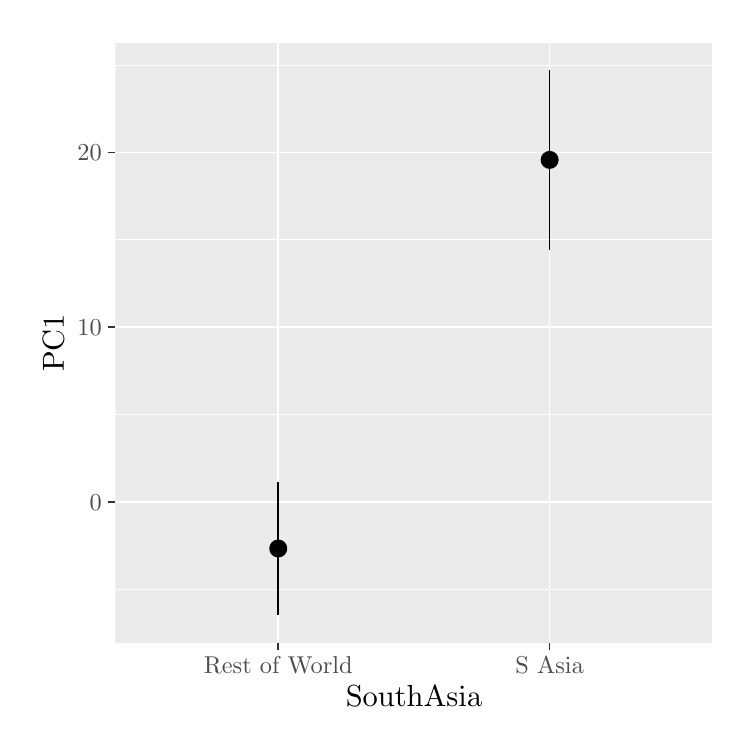
\begin{tikzpicture}[x=1pt,y=1pt]
\definecolor{fillColor}{RGB}{255,255,255}
\path[use as bounding box,fill=fillColor,fill opacity=0.00] (0,0) rectangle (252.94,252.94);
\begin{scope}
\path[clip] (  0.00,  0.00) rectangle (252.94,252.94);
\definecolor{drawColor}{RGB}{255,255,255}
\definecolor{fillColor}{RGB}{255,255,255}

\path[draw=drawColor,line width= 0.6pt,line join=round,line cap=round,fill=fillColor] (  0.00,  0.00) rectangle (252.94,252.94);
\end{scope}
\begin{scope}
\path[clip] ( 31.71, 30.69) rectangle (247.44,247.45);
\definecolor{fillColor}{gray}{0.92}

\path[fill=fillColor] ( 31.71, 30.69) rectangle (247.44,247.45);
\definecolor{drawColor}{RGB}{255,255,255}

\path[draw=drawColor,line width= 0.3pt,line join=round] ( 31.71, 49.89) --
	(247.44, 49.89);

\path[draw=drawColor,line width= 0.3pt,line join=round] ( 31.71,113.07) --
	(247.44,113.07);

\path[draw=drawColor,line width= 0.3pt,line join=round] ( 31.71,176.25) --
	(247.44,176.25);

\path[draw=drawColor,line width= 0.3pt,line join=round] ( 31.71,239.42) --
	(247.44,239.42);

\path[draw=drawColor,line width= 0.6pt,line join=round] ( 31.71, 81.48) --
	(247.44, 81.48);

\path[draw=drawColor,line width= 0.6pt,line join=round] ( 31.71,144.66) --
	(247.44,144.66);

\path[draw=drawColor,line width= 0.6pt,line join=round] ( 31.71,207.83) --
	(247.44,207.83);

\path[draw=drawColor,line width= 0.6pt,line join=round] ( 90.55, 30.69) --
	( 90.55,247.45);

\path[draw=drawColor,line width= 0.6pt,line join=round] (188.61, 30.69) --
	(188.61,247.45);
\definecolor{drawColor}{RGB}{0,0,0}

\path[draw=drawColor,line width= 0.6pt,line join=round] ( 90.55, 40.54) -- ( 90.55, 88.93);

\path[draw=drawColor,line width= 0.6pt,line join=round] (188.61,172.72) -- (188.61,237.59);
\definecolor{fillColor}{RGB}{0,0,0}

\path[draw=drawColor,line width= 0.8pt,line join=round,line cap=round,fill=fillColor] ( 90.55, 64.74) circle (  2.85);

\path[draw=drawColor,line width= 0.8pt,line join=round,line cap=round,fill=fillColor] (188.61,205.16) circle (  2.85);
\end{scope}
\begin{scope}
\path[clip] (  0.00,  0.00) rectangle (252.94,252.94);
\definecolor{drawColor}{gray}{0.30}

\node[text=drawColor,anchor=base east,inner sep=0pt, outer sep=0pt, scale=  0.88] at ( 26.76, 78.45) {0};

\node[text=drawColor,anchor=base east,inner sep=0pt, outer sep=0pt, scale=  0.88] at ( 26.76,141.63) {10};

\node[text=drawColor,anchor=base east,inner sep=0pt, outer sep=0pt, scale=  0.88] at ( 26.76,204.80) {20};
\end{scope}
\begin{scope}
\path[clip] (  0.00,  0.00) rectangle (252.94,252.94);
\definecolor{drawColor}{gray}{0.20}

\path[draw=drawColor,line width= 0.6pt,line join=round] ( 28.96, 81.48) --
	( 31.71, 81.48);

\path[draw=drawColor,line width= 0.6pt,line join=round] ( 28.96,144.66) --
	( 31.71,144.66);

\path[draw=drawColor,line width= 0.6pt,line join=round] ( 28.96,207.83) --
	( 31.71,207.83);
\end{scope}
\begin{scope}
\path[clip] (  0.00,  0.00) rectangle (252.94,252.94);
\definecolor{drawColor}{gray}{0.20}

\path[draw=drawColor,line width= 0.6pt,line join=round] ( 90.55, 27.94) --
	( 90.55, 30.69);

\path[draw=drawColor,line width= 0.6pt,line join=round] (188.61, 27.94) --
	(188.61, 30.69);
\end{scope}
\begin{scope}
\path[clip] (  0.00,  0.00) rectangle (252.94,252.94);
\definecolor{drawColor}{gray}{0.30}

\node[text=drawColor,anchor=base,inner sep=0pt, outer sep=0pt, scale=  0.88] at ( 90.55, 19.68) {Rest of World};

\node[text=drawColor,anchor=base,inner sep=0pt, outer sep=0pt, scale=  0.88] at (188.61, 19.68) {S Asia};
\end{scope}
\begin{scope}
\path[clip] (  0.00,  0.00) rectangle (252.94,252.94);
\definecolor{drawColor}{RGB}{0,0,0}

\node[text=drawColor,anchor=base,inner sep=0pt, outer sep=0pt, scale=  1.10] at (139.58,  7.64) {SouthAsia};
\end{scope}
\begin{scope}
\path[clip] (  0.00,  0.00) rectangle (252.94,252.94);
\definecolor{drawColor}{RGB}{0,0,0}

\node[text=drawColor,rotate= 90.00,anchor=base,inner sep=0pt, outer sep=0pt, scale=  1.10] at ( 13.08,139.07) {PC1};
\end{scope}
\end{tikzpicture}
